\addcontentsline{toc}{section}{CAPÍTULO X}
\chapter{EVALUACIÓN DE RESULTADOS}

\section{Resultados del \textit{benchmark}}

El \textit{benchmark} de cinco modelos sobre 101 liquidaciones (505 evaluaciones) reveló diferencias sustantivas en la capacidad de discriminación, la profundidad del análisis y la viabilidad económica de cada modelo.

 \textbf{Claude Sonnet 4 discrimina mejor que los demás.} Con una desviación estándar de 20.1 en los puntajes de riesgo, Sonnet separa los casos de bajo riesgo de los de alto riesgo con la mayor amplitud. Su distribución entre bandas fue la más equilibrada: 24.8 \% bajo, 44.6 \% medio, 30.7 \% alto. La hipótesis del equipo es que Sonnet, al ser un modelo optimizado para eficiencia, emite juicios más concisos y binarios. Opus, GPT-5.4 y Gemini, al generar análisis más detallados, encuentran más puntos de fricción en cada liquidación y terminan inflando los puntajes de forma sistemática.

\begin{figure}[H]
\centering
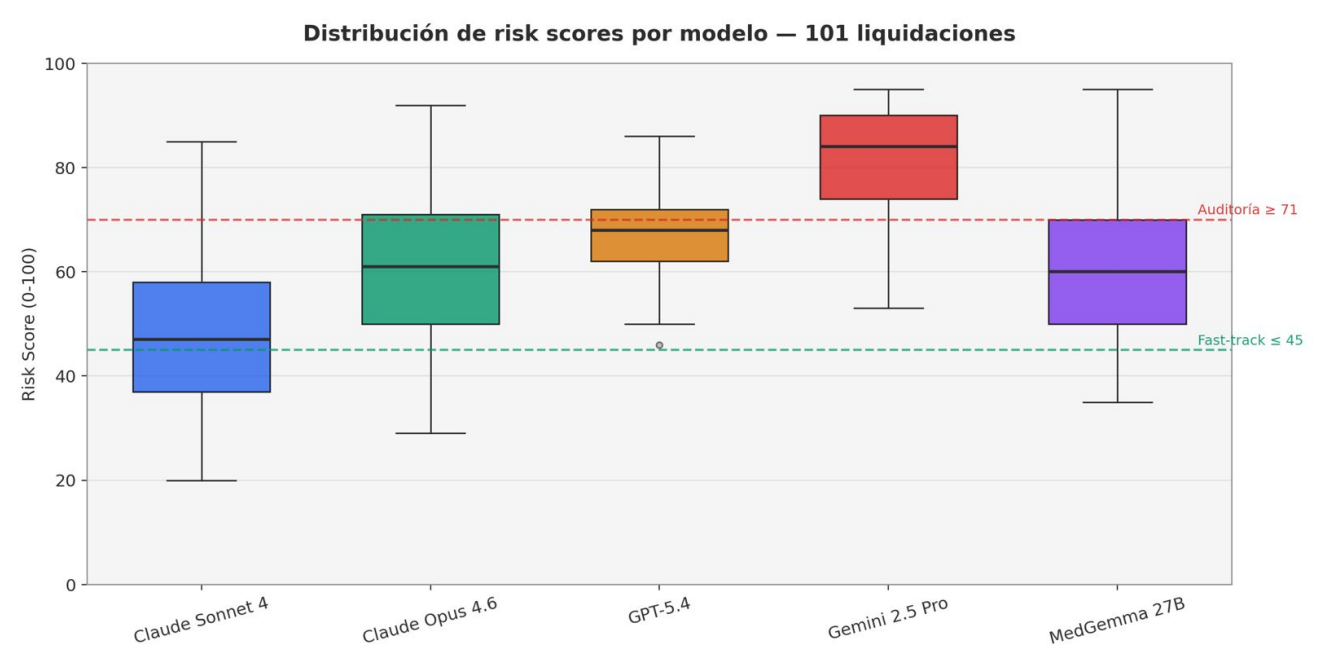
\includegraphics[width=0.96\textwidth,height=0.72\textheight,keepaspectratio]{images/p46_figure_1.png}
\caption{Distribución de puntajes de riesgo por modelo.}
\end{figure}

\textbf{GPT-5.4 resulta inviable para fast-track.} Con 0 \% de liquidaciones clasificadas como bajo riesgo, una desviación estándar de 8.8 y un puntaje mínimo de 42, GPT-5.4 trata todas las liquidaciones como si fueran de riesgo medio-alto. Su media de 69.3 está prácticamente en la frontera de auditoría completa. Un sistema que escala todo a revisión humana no aporta valor operativo. El hallazgo es relevante porque GPT-5.4 demostró buena profundidad clínica, lo que sugiere que su problema no es la falta de capacidad analítica sino un sesgo sistemático hacia la sobrepenalización.

Los tres modelos restantes resultaron inviables como modelo único, aunque por razones distintas. Opus genera el análisis más profundo del \textit{benchmark}, pero con solo 3.1 \% de fast-track y un costo 10x, funciona como segundo nivel, no como \textit{screening}. MedGemma, pese a su entrenamiento médico, obtuvo la menor profundidad y quedó limitado por su ventana de 8,192 \textit{tokens} y la necesidad de GPU dedicada. Gemini fue el más barato y el más confiable en \textit{parsing}, pero clasificó el 96 \% de los casos como de alto riesgo.

\begin{figure}[H]
\centering
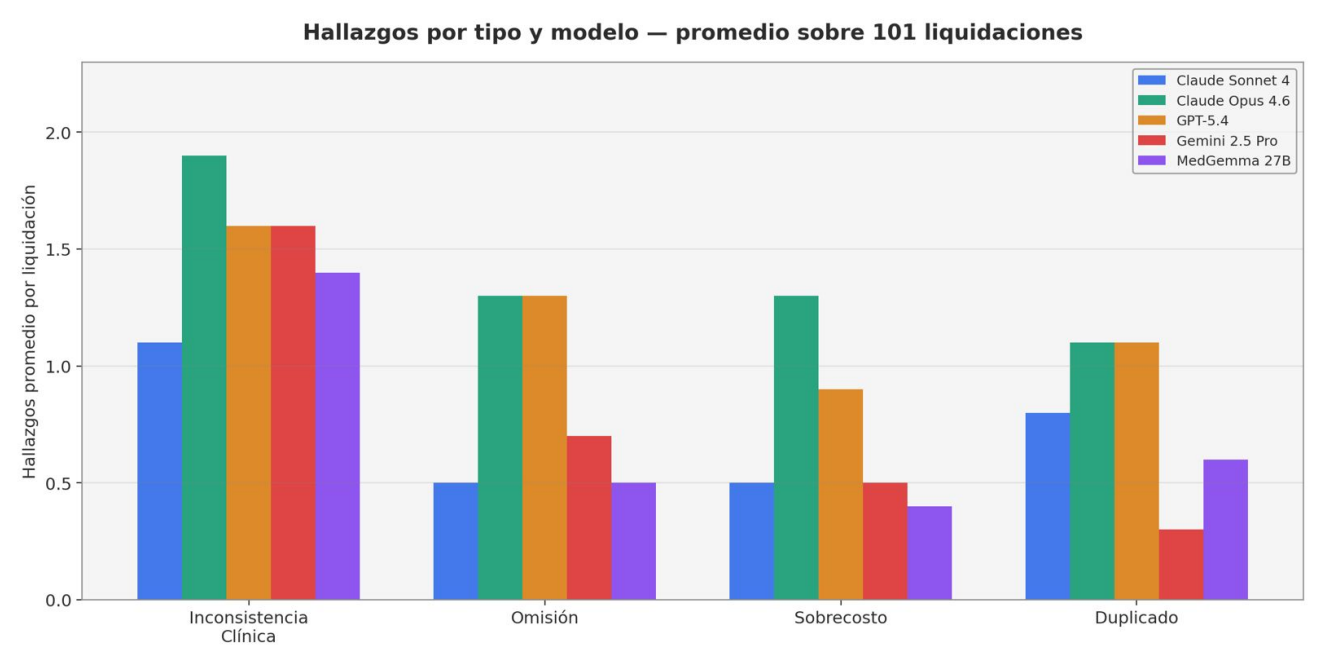
\includegraphics[width=0.96\textwidth,height=0.72\textheight,keepaspectratio]{images/p47_figure_1.png}
\caption{Promedio de hallazgos por liquidación, por tipo y modelo.}
\end{figure}

\textbf{Análisis de \textit{confounding}: ¿el volumen de ítems infla el puntaje?} Para cuantificar este efecto, se calculó la correlación entre el número total de ítems por liquidación y el \textit{risk score} asignado por cada modelo se presentan en la Tabla~\ref{tab:correlacion-items-risk-score}

\begin{table}[H]
    \centering
    \caption{Correlación entre número de ítems por liquidación y
    \textit{risk score}}
    \label{tab:correlacion-items-risk-score}

    \footnotesize
    \setlength{\tabcolsep}{7pt}
    \renewcommand{\arraystretch}{1.2}

    \begin{tabular}{
        l
        c
        c
        c
        c
        c
    }
        \toprule
        \textbf{Modelo}
        & \textbf{n}
        & \textbf{Pearson r}
        & \textbf{p-value}
        & \textbf{Spearman $\rho$}
        & \textbf{p-value} \\
        \midrule

        Claude Sonnet 4 & 101 & $-0.21$ & 0.035 & $-0.45$ & $< 0.001$ \\
        Claude Opus 4.6 & 98  & 0.04    & 0.732 & $-0.19$ & 0.064 \\
        GPT-5.4         & 99  & 0.03    & 0.808 & $-0.28$ & 0.004 \\
        Gemini 2.5 Pro  & 101 & $-0.07$ & 0.484 & $-0.28$ & 0.003 \\
        MedGemma 27B    & 101 & $-0.08$ & 0.427 & $-0.32$ & $< 0.001$ \\

        \bottomrule
    \end{tabular}
\end{table}

Ningún modelo muestra correlación positiva significativa entre volumen y \textit{score}. Sonnet, el modelo seleccionado para \textit{screening}, presenta una correlación negativa. Esto descarta la hipótesis de que la capacidad discriminativa de Sonnet sea un artefacto de la complejidad del caso. La discriminación por sigma es una condición necesaria, pero no suficiente: la validación de precisión a nivel de hallazgo requiere un piloto con auditor real.

\section{\textit{pipeline} integrado}

El \textit{pipeline} completo (Fase 1 + Fase 2 con estrategia escalonada, \textit{prompts} de producción e \textit{Identity Vault} activo) se ejecutó sobre las 101 liquidaciones del \textit{dataset} . A diferencia de las proyecciones de la sección 7.10, esta ejecución invocó el LLM real con la configuración de producción.

La distribución real de decisiones fue:

\begin{table}[H]
    \centering
    \caption{Distribución real de decisiones del \textit{pipeline} integrado}
    \label{tab:distribucion-decisiones-pipeline}

    \setlength{\tabcolsep}{10pt}
    \renewcommand{\arraystretch}{1.25}

    \begin{tabular}{
        l
        c
        c
        c
    }
        \toprule
        \textbf{Categoría}
        & \textbf{Cantidad}
        & \textbf{\% real}
        & \textbf{Proyección Sección~\ref{sec:resultados-preliminares}} \\
        \midrule

        \texttt{FAST\_TRACK}
        & 66
        & 65.3\,\%
        & 55--65\,\% \\

        \texttt{REVISION\_RAPIDA}
        & 9
        & 8.9\,\%
        & 15--20\,\% \\

        \texttt{AUDITORIA\_COMPLETA}
        & 26
        & 25.7\,\%
        & 10--15\,\% \\

        \texttt{RECHAZO\_ADMINISTRATIVO}
        & 0
        & 0.0\,\%
        & 3--5\,\% \\

        \bottomrule
    \end{tabular}
\end{table}

La tasa de recomendación de fast-track (65.3 \%) se ubica en el extremo superior del rango proyectado y casi triplica el 24.8 \% del \textit{benchmark} con Sonnet aislado. Esta tasa refleja la clasificación del \textit{pipeline}; la tasa efectiva de fast-track depende de la aceptación del auditor, un factor no medido en este alcance. La categoría AUDITORIA\_COMPLETA es mayor a lo proyectado porque el

LLM con \textit{prompts} de producción detecta inconsistencias clínicas que la simulación con puntajes fijos no capturaba. No hubo rechazos administrativos.

Los \textit{prompts} de producción y el pre-filtrado de Fase 1 produjeron un desplazamiento medible en la distribución de \textit{scores} de Sonnet en la tabla~\ref{tab:cambio-distribucion-scores-sonnet}:

\begin{table}[H]
    \centering
    \caption{Cambio en la distribución de \textit{scores} de Sonnet}
    \label{tab:cambio-distribucion-scores-sonnet}

    \footnotesize
    \setlength{\tabcolsep}{6pt}
    \renewcommand{\arraystretch}{1.25}

    \begin{tabular}{
        p{0.25\textwidth}
        p{0.25\textwidth}
        p{0.23\textwidth}
        p{0.13\textwidth}
    }
        \toprule
        \textbf{Métrica}
        & \textbf{\textit{Benchmark} (Sonnet aislado)}
        & \textbf{\textit{Pipeline} integrado}
        & \textbf{Cambio} \\
        \midrule

        Media del \textit{risk score}
        & 48.1
        & 38.6
        & $-9.5$ \\

        $\sigma$ del \textit{risk score}
        & 20.1
        & 24.9
        & $+4.8$ \\

        Mediana
        & ---
        & 25.0
        & --- \\

        Tasa de recomendación \textit{fast-track}
        & 24.8\,\% (umbral $\leq 30$)
        & 65.3\,\% (umbral $\leq 45$)
        & $+40.5$ pp \\

        Errores de \textit{parsing}
        & ---
        & 0 (Sonnet) / 0 (Opus)
        & --- \\

        \bottomrule
    \end{tabular}

    \vspace{2mm}

    \begin{minipage}{0.94\textwidth}
        \footnotesize
        \textit{Nota:} Los umbrales difieren entre ambas configuraciones
        ($\leq 30$ frente a $\leq 45$). La descomposición de factores se
        presenta en la tabla~\ref{tab:estudio-ablacion}
    \end{minipage}
\end{table}

Nota: Los umbrales difieren entre ambas configuraciones ($\leq$ 30 vs. $\leq$ 45). La descomposición de factores se presenta más adelante en la tabla~\ref{tab:estudio-ablacion}

De los 101 \textit{claims}, 33 (32.7 \%) fueron escalados a Opus. Los motivos de escalación, que pueden coexistir en un mismo \textit{claim}, fueron: \textit{score} Sonnet > 45 (26 \textit{claims}), hallazgo de alta severidad por inconsistencia clínica (14 \textit{claims}), y costo total > S/5,000 con ítems en revisión (9 \textit{claims}). Opus procesó los 33 \textit{claims} sin errores de \textit{parsing}, con un tiempo promedio de 25.2 segundos por caso.

\begin{figure}[H]
\centering
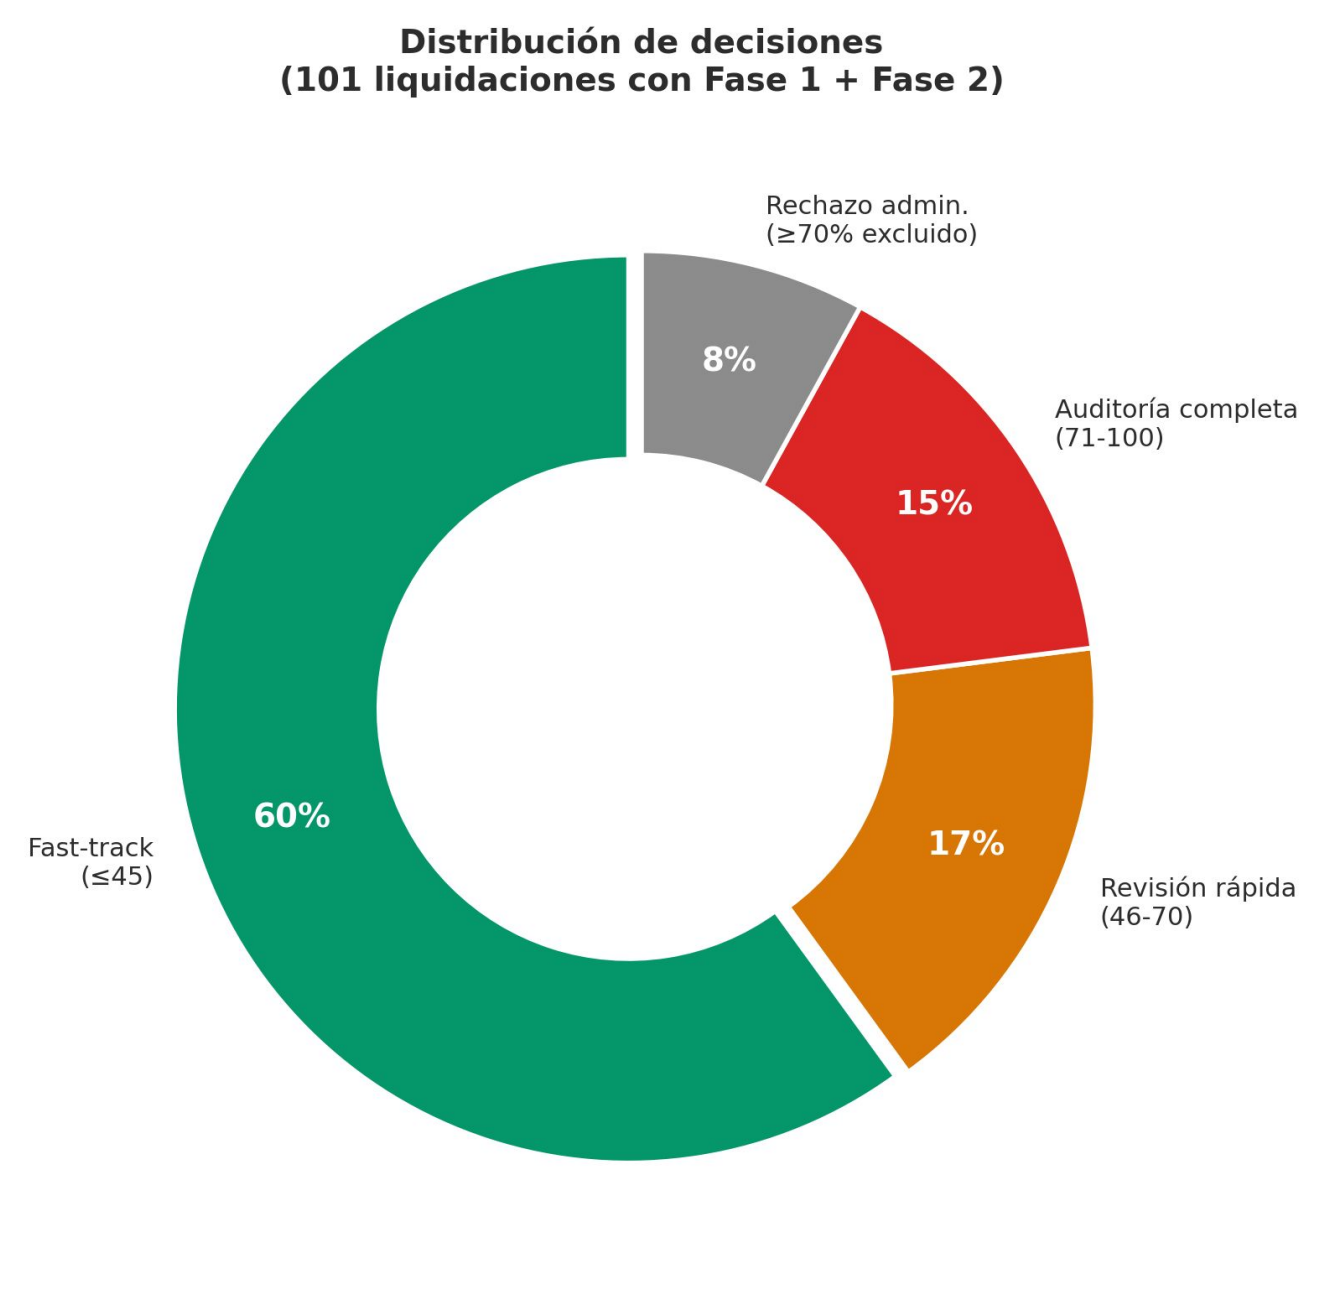
\includegraphics[width=0.96\textwidth,height=0.72\textheight,keepaspectratio]{images/p50_figure_1.png}
\caption{Distribución real de decisiones del \textit{pipeline} integrado.}
\label{p50_figure_1}
\end{figure}

\textbf{Nota sobre la comparación de umbrales.} La tasa de fast-track del \textit{benchmark} (24.8 \%) utilizó un umbral de $\leq$ 30, mientras que el \textit{pipeline} de producción emplea $\leq$ 45. Esta diferencia es el factor dominante en la mejora observada. Un estudio de ablación permite descomponer la contribución de cada factor:

\begin{table}[H]
    \centering
    \caption{Estudio de ablación de la mejora en la tasa de \textit{fast-track}}
    \label{tab:estudio-ablacion}

    \footnotesize
    \setlength{\tabcolsep}{6pt}
    \renewcommand{\arraystretch}{1.25}

    \begin{tabular}{
        p{0.27\textwidth}
        c
        p{0.16\textwidth}
        c
        c
        c
    }
        \toprule
        \textbf{Configuración}
        & \textbf{Umbral}
        & \textbf{\textit{Prompts}}
        & \textbf{Fase 1}
        & \textbf{Media del \textit{score}}
        & \textbf{\textit{Fast-track}} \\
        \midrule

        \textit{Benchmark} original
        & $\leq 30$
        & \textit{Benchmark}
        & No
        & 48.1
        & 24.8\,\% \\

        Solo cambio de umbral
        & $\leq 45$
        & \textit{Benchmark}
        & No
        & 48.1
        & 66.3\,\% \\

        \textit{Prompts} de producción, sin Fase 1
        & $\leq 45$
        & Producción
        & No
        & 37.9
        & 72.3\,\% \\

        \textit{Pipeline} completo
        & $\leq 45$
        & Producción
        & Sí
        & 38.6
        & 65.3\,\% \\

        \bottomrule
    \end{tabular}
\end{table}

El estudio de ablación descompone la mejora en tres efectos independientes:

\noindent \textbf{1. Cambio de umbral:} +41.6 pp.

\noindent \textbf{2. \textit{Prompts} de producción:} +6.0 pp.

\noindent \textbf{3. Fase 1 (pre-filtrado contractual):} -7.0 pp.

El valor de Fase 1 no está en aumentar la tasa de fast-track, sino en mejorar la calidad de la discriminación. Los \textit{claims} clasificados como fast-track con el \textit{pipeline} completo tienen mayor consistencia clínica verificada que los que habrían calificado solo con \textit{prompts} de producción.

El costo total de API fue de \$12.00 (\$2.83 para las 101 llamadas a Sonnet + \$9.17 para las 33 llamadas a Opus), con un tiempo total de ejecución de 38.9 minutos. El costo por \textit{claim} promedio fue de \$0.12.

Aplicando los tiempos estimados de revisión del auditor (1 min para fast-track, 10 min para revisión rápida, 45 min para auditoría completa), el tiempo total proyectado del lote sería de aproximadamente 21 horas, frente a las 75.8 horas del proceso manual, una reducción del 72 \%.

\section{Hallazgos clínicos de alto impacto}

Más allá de las métricas de distribución, el valor operativo del sistema se ilustra con los hallazgos que la Fase 2 señaló como candidatos a investigación durante el \textit{benchmark}. En cinco expedientes, el LLM identificó patrones de facturación que ameritan revisión por un auditor, por un monto acumulado superior a S/70,000. Ninguno de estos hallazgos constituye una determinación de fraude o de error, pero sí demuestran la capacidad del sistema para priorizar los casos que merecen atención humana.

Dos casos ilustran los patrones que el sistema escala para revisión humana. En una angioplastia valorada en aproximadamente S/39,460, los stents coronarios aparecen registrados como devueltos en el sistema de farmacia, pero el honorario por el procedimiento de implantación se mantuvo facturado. Un patrón similar se observó en una cirugía de fémur valorada en aproximadamente S/31,177, en la que la prótesis fue revertida, pero el cobro del procedimiento persistió. La inconsistencia entre la reversión del insumo de alto costo y el mantenimiento del honorario quirúrgico puede tener explicaciones operativas legítimas, pero también es consistente con patrones conocidos de facturación de procedimientos no completados.

En el ámbito de inconsistencias clínicas, el sistema detectó un expediente de un paciente geriátrico hospitalizado por neumonía donde se facturaron cero antibióticos, cero imágenes diagnósticas y cero broncodilatadores, una omisión farmacológica incompatible con el diagnóstico. En otro caso, alertó sobre la ausencia de profilaxis antitrombótica en una cirugía abdominal de una paciente de 83 años, una omisión que constituye un riesgo clínico grave según protocolos estándar.

Estos hallazgos ilustran que la Fase 2 aporta un valor que excede la verificación contractual de la Fase 1: la capacidad de cruzar el diagnóstico, los servicios facturados y los protocolos médicos esperados para señalar discrepancias que ameritan revisión humana.

\section{Validación con \textit{Golden Set}}

El \textit{Golden Set} de 17 liquidaciones, cuyas clasificaciones esperadas fueron validadas por un auditor médico externo al equipo, constituye el mecanismo de regresión y calibración del \textit{pipeline}. No es un conjunto de validación independiente, pero cumple una función operativa esencial: detectar degradaciones ante cambios en el sistema.

\textbf{Nivel 1: \textit{Routing} de Fase 1} Los 17 \textit{tests} parametrizados de test\_routing\_matches\_expected verifican que cada liquidación del \textit{Golden Set} recibe el \textit{routing} correcto. Los \textit{tests} de elegibilidad y cobertura también pasan.

\textbf{Nivel 2: Motor de decisión} Seis \textit{tests} simulan puntajes de Fase 2 para verificar que el motor de decisión produce las categorías esperadas. Se confirma, entre otros puntos, que el umbral de 45 es inclusivo y que la edad avanzada no genera una penalización automática.

\textbf{Nivel 3: Proyección de tasa} test\_projected\_rate\_meets\_target ejecuta Fase 1 sobre las 101 liquidaciones completas, simula Fase 2 y verifica que la tasa de fast-track se encuentra entre 55 \% y 75 \%.

\textbf{Diagnóstico de concordancia} La ejecución real del \textit{pipeline} logró una concordancia de 10/17 (58.8 \%) con las clasificaciones esperadas del \textit{Golden Set}. Esta cifra no constituye una métrica de rendimiento generalizable; su valor es diagnóstico. Revela que la tasa de falsos negativos fue del 0 \% y que los 7 \textit{mismatches} corresponden exclusivamente a sobre-escalaciones donde el LLM detectó inconsistencias clínicas que no eran evidentes en la revisión inicial del auditor.

\textbf{Estabilidad de umbrales \textit{(Leave-One-Out)}} Para evaluar si los umbrales dependen de algún caso individual del \textit{Golden Set}, se implementó un análisis \textit{leave-one-out}. Los 17 \textit{claims} pasan las verificaciones, confirmando que ningún caso individual es pivotal para la determinación del umbral.

\section{Análisis de costos}

El análisis económico compara tres estrategias de procesamiento con el costo manual tabla~\ref{tab:comparacion-estrategias-procesamiento}:

\begin{table}[H]
    \centering
    \caption{Comparación de estrategias de procesamiento}
    \label{tab:comparacion-estrategias-procesamiento}

    \footnotesize
    \setlength{\tabcolsep}{6pt}
    \renewcommand{\arraystretch}{1.3}

    \begin{tabular}{
        p{0.28\textwidth}
        p{0.23\textwidth}
        p{0.16\textwidth}
        p{0.25\textwidth}
    }
        \toprule
        \textbf{Estrategia}
        & \textbf{Costo por lote (101 \textit{claims})}
        & \textbf{Tiempo de API}
        & \textbf{Observación} \\
        \midrule

        Claude Sonnet 4 exclusivo
        & USD 2.83
        & $\sim 27.8$ min
        & Triaje eficiente, con menor profundidad clínica. \\

        Claude Opus 4.6 exclusivo
        & USD 28.08
        & $\sim 84.5$ min
        & Máxima profundidad, con un costo aproximadamente 10 veces mayor. \\

        Estrategia escalonada (Sonnet + Opus)
        & USD 12.00
        & $\sim 38.9$ min
        & Balance entre costo y calidad. \\

        Auditoría manual
        & 75.8 h $\times$ costo del auditor
        & 75.8 h
        & Línea base actual. \\

        \bottomrule
    \end{tabular}
\end{table}


El costo de la estrategia escalonada (\$12.00 por lote) representa menos del 0.001 \% del valor promedio de un lote hospitalario. El costo de API no es el factor limitante para la viabilidad económica del sistema; lo son la adopción por parte del auditor y la integración con los sistemas existentes.

\section{Cumplimiento de objetivos}

La siguiente tabla~\ref{tab:cumplimiento-objetivos} cruza cada objetivo específico con los resultados obtenidos:

\begin{table}[H]
    \centering
    \caption{Cumplimiento de los objetivos del proyecto}
    \label{tab:cumplimiento-objetivos}

    \footnotesize
    \setlength{\tabcolsep}{6pt}
    \renewcommand{\arraystretch}{1.3}

    \begin{tabular}{
        p{0.26\textwidth}
        p{0.19\textwidth}
        p{0.33\textwidth}
        p{0.16\textwidth}
    }
        \toprule
        \textbf{Objetivo}
        & \textbf{Meta}
        & \textbf{Resultado}
        & \textbf{Estado} \\
        \midrule

        OE1: Tasa de recomendación de \textit{fast-track}
        & 50--60\,\%
        & 65.3\,\% (66/101)
        & Cumplido \\

        OE2: Control de falsos positivos
        & Por definir en producción
        & No estimable con la evidencia disponible
        & No medido \\

        OE3: Tiempo por liquidación
        & $\leq 5$ min
        & $< 1$ min para \textit{fast-track};
          $\sim 17$ s de procesamiento del LLM
        & Cumplido \\

        Derivado: reducción del tiempo por lote
        & $\geq 40\,\%$
        & 57--72\,\%, según el escenario
        & Cumplido (estimado) \\

        Derivado: reducción del MLR
        & 1--2 puntos porcentuales
        & No medible sin un piloto real
        & No medido \\

        \bottomrule
    \end{tabular}
\end{table}

 \textbf{Sensibilidad de la reducción de tiempo.} La reducción de tiempo por lote depende de la confianza del auditor en el sistema. El siguiente (Tabla~\ref{tab:sensibilidad-reduccion-tiempo}) análisis muestra cómo varía bajo tres escenarios de adopción:

\begin{table}[H]
    \centering
    \caption{Sensibilidad de la reducción del tiempo por lote}
    \label{tab:sensibilidad-reduccion-tiempo}

    \footnotesize
    \setlength{\tabcolsep}{5pt}
    \renewcommand{\arraystretch}{1.25}

    \begin{tabular}{
        l
        c
        c
        c
        c
        c
    }
        \toprule
        \textbf{Escenario}
        & \textbf{t(\textit{fast-track})}
        & \textbf{t(rev. rápida)}
        & \textbf{t(aud. completa)}
        & \textbf{Total del lote}
        & \shortstack{\textbf{Reducción}\\\textbf{vs. 75.8 h}} \\
        \midrule

        Optimista
        & 1 min
        & 10 min
        & 45 min
        & 21.0 h
        & 72\,\% \\

        Conservador
        & 5 min
        & 15 min
        & 45 min
        & 27.2 h
        & 64\,\% \\

        Pesimista
        & 10 min
        & 20 min
        & 45 min
        & 32.5 h
        & 57\,\% \\

        \bottomrule
    \end{tabular}
\end{table}

Los tres escenarios superan la meta del 40 \%. Sin embargo, la reducción real depende de la confianza del auditor en el sistema, un factor que solo puede medirse en un piloto controlado.

 \textbf{Sensibilidad de la tasa efectiva de fast-track.} La tasa de recomendación de fast-track (65.3 \%) se convierte en tasa efectiva solo cuando el auditor acepta la recomendación:

\begin{table}[H]
    \centering
    \caption{Sensibilidad de la tasa efectiva de \textit{fast-track}}
    \label{tab:sensibilidad-fast-track-efectivo}

    \footnotesize
    \setlength{\tabcolsep}{7pt}
    \renewcommand{\arraystretch}{1.25}

    \begin{tabular}{
        p{0.32\textwidth}
        p{0.18\textwidth}
        p{0.16\textwidth}
        p{0.24\textwidth}
    }
        \toprule
        \textbf{Tasa de aceptación del auditor}
        & \textbf{\textit{Fast-track} efectivos}
        & \textbf{Tasa efectiva}
        & \textbf{Comparación con la meta de 50--60\,\%} \\
        \midrule

        90\,\%
        & 59
        & 58.8\,\%
        & Dentro de la meta \\

        80\,\%
        & 53
        & 52.2\,\%
        & Dentro de la meta \\

        70\,\%
        & 46
        & 45.7\,\%
        & Por debajo \\

        60\,\%
        & 40
        & 39.2\,\%
        & Por debajo \\

        \bottomrule
    \end{tabular}
\end{table}

Con una aceptación del 77 \% o superior, la tasa efectiva se mantiene dentro de la meta del 50 \%. Esta tasa de aceptación es plausible, pero solo puede confirmarse en un piloto con auditor real.

En síntesis, el MVP demuestra que la arquitectura funciona y que las proyecciones son favorables. Lo que no demuestra, porque no puede hacerlo dentro del alcance académico, es que el sistema produce los resultados esperados cuando un auditor real procesa un lote real con datos de producción. Esa validación requiere un piloto.
